\documentclass[sigconf,anonymous]{acmart}

\usepackage{microtype}

% Submission metadata (anonymized)
\setcopyright{none}
\settopmatter{printacmref=true, printfolios=false}
\pagestyle{plain}
\acmConference[ICAIF 2026]{Proceedings of ACM on AI in Finance (ICAIF 2026)}{2026}{}
\copyrightyear{2026}
\acmYear{2026}

% ACM concepts block (mandatory for ACM two-column templates over two pages)
\begin{CCSXML}
<ccs2012>
  <concept>
    <concept_id>10002951.10002952.10002953</concept_id>
    <concept_desc>Computing methodologies~Machine learning</concept_desc>
    <concept_significance>500</concept_significance>
  </concept>
  <concept>
    <concept_id>10002951.10002950.10002967</concept_id>
    <concept_desc>Computer systems organization~Cloud computing</concept_desc>
    <concept_significance>300</concept_significance>
  </concept>
</ccs2012>
\end{CCSXML}
\ccsdesc[500]{Computing methodologies~Machine learning}
\ccsdesc[300]{Computer systems organization~Cloud computing}

% Packages
\usepackage{amsmath}
\usepackage{amsthm}
\usepackage{booktabs}
\usepackage{graphicx}
\usepackage{multirow}
\usepackage{xcolor}
\newtheorem{theorem}{Theorem}

% Typographic safety for long equations
\sloppy
\emergencystretch 1.5em

% Bib style
\bibliographystyle{ACM-Reference-Format}

\title{Diagnosing Conformal Prediction Failures Under Distribution Shift: A COVID-19 Case Study}

\begin{document}

\begin{abstract}
Conformal prediction coverage guarantees rely on exchangeability but can degrade severely under shift. We ask which deployed models fail before any test data is observed. On a temporal COVID-19 split of SALT supply-chain tasks and extensions to 11 additional domains, we find that \emph{SHAP concentration}---the fraction of SHAP mass on the top feature---strongly predicts coverage failure for gradient-boosted classifiers under covariate shift. Concentration alone is consistent with why coverage losses range from near-zero to over 70\% despite similar shift. We report 50-seed experiments, confirm a concentration--degradation relationship across 16 multiclass tasks (Spearman $\rho=0.853$, $p<0.001$), and show that standard shift detectors (MMD/C2ST/PSI) do not predict failure severity. A short exploratory decision rule uses SHAP concentration with a 40\% threshold and conservative ambiguity band. This work is associational: it identifies a model-specific pre-deployment risk signal tied to failure mechanism, not a universal causality law.
\end{abstract}

\keywords{Conformal prediction, covariate shift, SHAP, robustness, uncertainty quantification}

\setlength{\tabcolsep}{3pt}

\maketitle

\section{Introduction}
Conformal prediction offers finite-sample coverage guarantees under exchangeability, not under arbitrary shift.
In practice, shift is common, while practitioners need a \emph{pre-deployment} screen that flags likely breakdown before deployment.
Conformal extensions under covariate and adaptive settings provide useful guarantees under assumptions \citep{barber2023conformal,tibshirani2019conformal,zaffran2022adaptive},
but do not by themselves provide a task-level pre-deployment severity signal.
We evaluate whether the concentration of feature reliance in a model is such a screen.

\section{Related Work}
Shift detectors can identify distribution drift but may not prioritize which models fail severely \citep{koh2021wilds,malinin2021shifts,gulrajani2020search}.
APS and adaptive conformal methods capture performance under non-stationarity \citep{romano2020classification,gibbs2021adaptive}, while attribution methods provide model-level interpretability \citep{lundberg2017unified,lundberg2020local}.
We compare these ideas by testing whether attribution structure predicts \emph{severity} of conformal degradation before test-time data is observed.

\textbf{Contributions.}
\begin{itemize}
  \item We evaluate a model-level diagnostic, \textit{SHAP concentration}, as an early-warning metric before test observation.
  \item We prove a monotone score-inflation mechanism for APS under high concentration on a shifted feature.
  \item We validate across 8 SALT tasks with heavy temporal shift, then extend to 16 multiclass tasks across 9 domains.
  \item We benchmark against baseline diagnostics and show that shift detectors predict shift existence but not degradation severity.
\end{itemize}

\section{Setup}
\subsection{Data and Splits}
We use the SALT benchmark (8 classification tasks) with aligned temporal splits:
\begin{itemize}
  \item Train: before Feb 2020, Val: Feb--Jul 2020, Test: after Jul 2020.
\end{itemize}
For external tests, we use 11 datasets across 10 domains. Excluding binary tasks yields 8 external multiclass datasets, and together with the 8 multiclass SALT tasks this gives the primary endpoint of $n=16$ multiclass tasks across 9 domains (SALT counts as one domain).

We compute SHAP concentration only from validation data:
\begin{equation}
  C = \frac{\phi_1}{\sum_{j=1}^{p} \phi_j},
\end{equation}
where $\phi_j$ is mean absolute SHAP for feature $j$ and $\phi_1$ is top-ranked feature SHAP. All models use the same pipeline with 50 random seeds; we report mean coverage, 95\% CI, and Wilcoxon tests.

\subsection{Conformal Protocol}
We use Adaptive Prediction Sets (APS) with $\alpha=0.1$ and target coverage $1-\alpha=0.9$. We use a non-randomized variant. We run 50 seeds for all SALT tasks and 10--50 seeds where available for external validation.

\section{Why Concentration Could Matter}
Two tasks share near-zero feature overlap, yet one loses little coverage and another loses over 70\%. This indicates that shift size alone is insufficient and that dependence geometry matters. Jaccard overlap is a coarse proxy, while concentration distinguishes how concentrated the 
model's dependence becomes on dominant features.
Concretely, if a shifted feature absorbs mass in the prediction ranking, APS can become more conservative on the true label despite similar observed turnover.

\section{Theory}
For a $K$-class classifier, APS score is the mass assigned at or above the true label.

\begin{theorem}[Score inflation under concentrated shift]
\label{thm:score_inflation}
Consider
\[
\hat p(y\mid x)=C\cdot g(y\mid x_1)+(1-C)\cdot h(y\mid x_{\setminus 1}),\quad K\ge3,
\]
with concentrated misclassification on $x_1$ under shift:
$g(y^\ast\mid x_1^{\text{test}})\le \epsilon<1/K$.
If the residual term is exchangeable between calibration and test, then APS scores
shift to larger values as $C$ increases and coverage upper bounds are non-increasing in $C$.
\end{theorem}

Theorem~\ref{thm:score_inflation} formalizes a mechanism: more mass on one shifted feature increases true-label score requirements, so prediction sets grow and coverage degrades. A full derivation appears in the paper code repository and experimental notebook.

\section{Empirical Findings}

\subsection{SALT Tasks: large variation under the same shift}

\begin{table*}[t]
\centering
\caption{Coverage degradation on SALT (50 seeds).}
\label{tab:salt}
\small
\setlength{\tabcolsep}{4pt}
\begin{tabular}{lccccc}
\toprule
Task & \#Cls & Val Coverage & Test Coverage & Drop & SHAP $C$ \\
\midrule
s-shipcond & 45 & 93.5 & 21.8 & 71.6 & 50.7 \\
s-group    & 462 & 83.6 & 12.4 & 71.2 & 47.3 \\
s-payterms & 135 & 90.8 & 13.7 & 77.1 & 54.2 \\
i-plant    & 35 & 92.0 & 81.4 & 10.6 & 23.9 \\
i-shippoint& 70 & 91.2 & 72.7 & 18.5 & 48.8 \\
s-incoterms & 13 & 95.5 & 87.0 & 8.5  & 23.7 \\
i-incoterms & 13 & 95.0 & 83.7 & 11.3 & 28.9 \\
s-office   & 25 & 99.9 & 99.9 & 0.1  & 42.6 \\
\bottomrule
\end{tabular}
\normalsize
\end{table*}

Despite identical COVID-era shift, coverage drops span 0.1--77.1\%, and concentration tracks these failures: catastrophic outcomes are concentrated, robust tasks are not.

\subsection{Concentration diagnostics}

\begin{table*}[t]
\centering
\caption{Diagnostics across SALT and external multiclass tasks.}
\label{tab:diagnostics}
\small
\setlength{\tabcolsep}{4pt}
\begin{tabular}{lcccc}
\toprule
Set & $n$ & Corr. with drop (Spearman $\rho$) & $p$ & Significance \\
\midrule
SALT multiclass ($K\ge 3$) & 8  & 0.833 & 0.010 & \textit{sig.} \\
SALT + cross-domain multiclass & 16 & 0.853 & $<0.001$ & \textit{significant} \\
Native FI concentration & 8  & 0.667 & 0.071 & \textit{weak} \\
Ensemble disagreement  & 8  & 0.452 & 0.260 & \textit{weak} \\
MMD / C2ST / PSI & 8  & $\le 0.19$ & $>0.6$ & \textit{not predictive} \\
\bottomrule
\end{tabular}
\normalsize
\end{table*}

SHAP concentration is strongest among evaluated pre-deployment diagnostics for these experiments.

\begin{figure}[t]
\centering
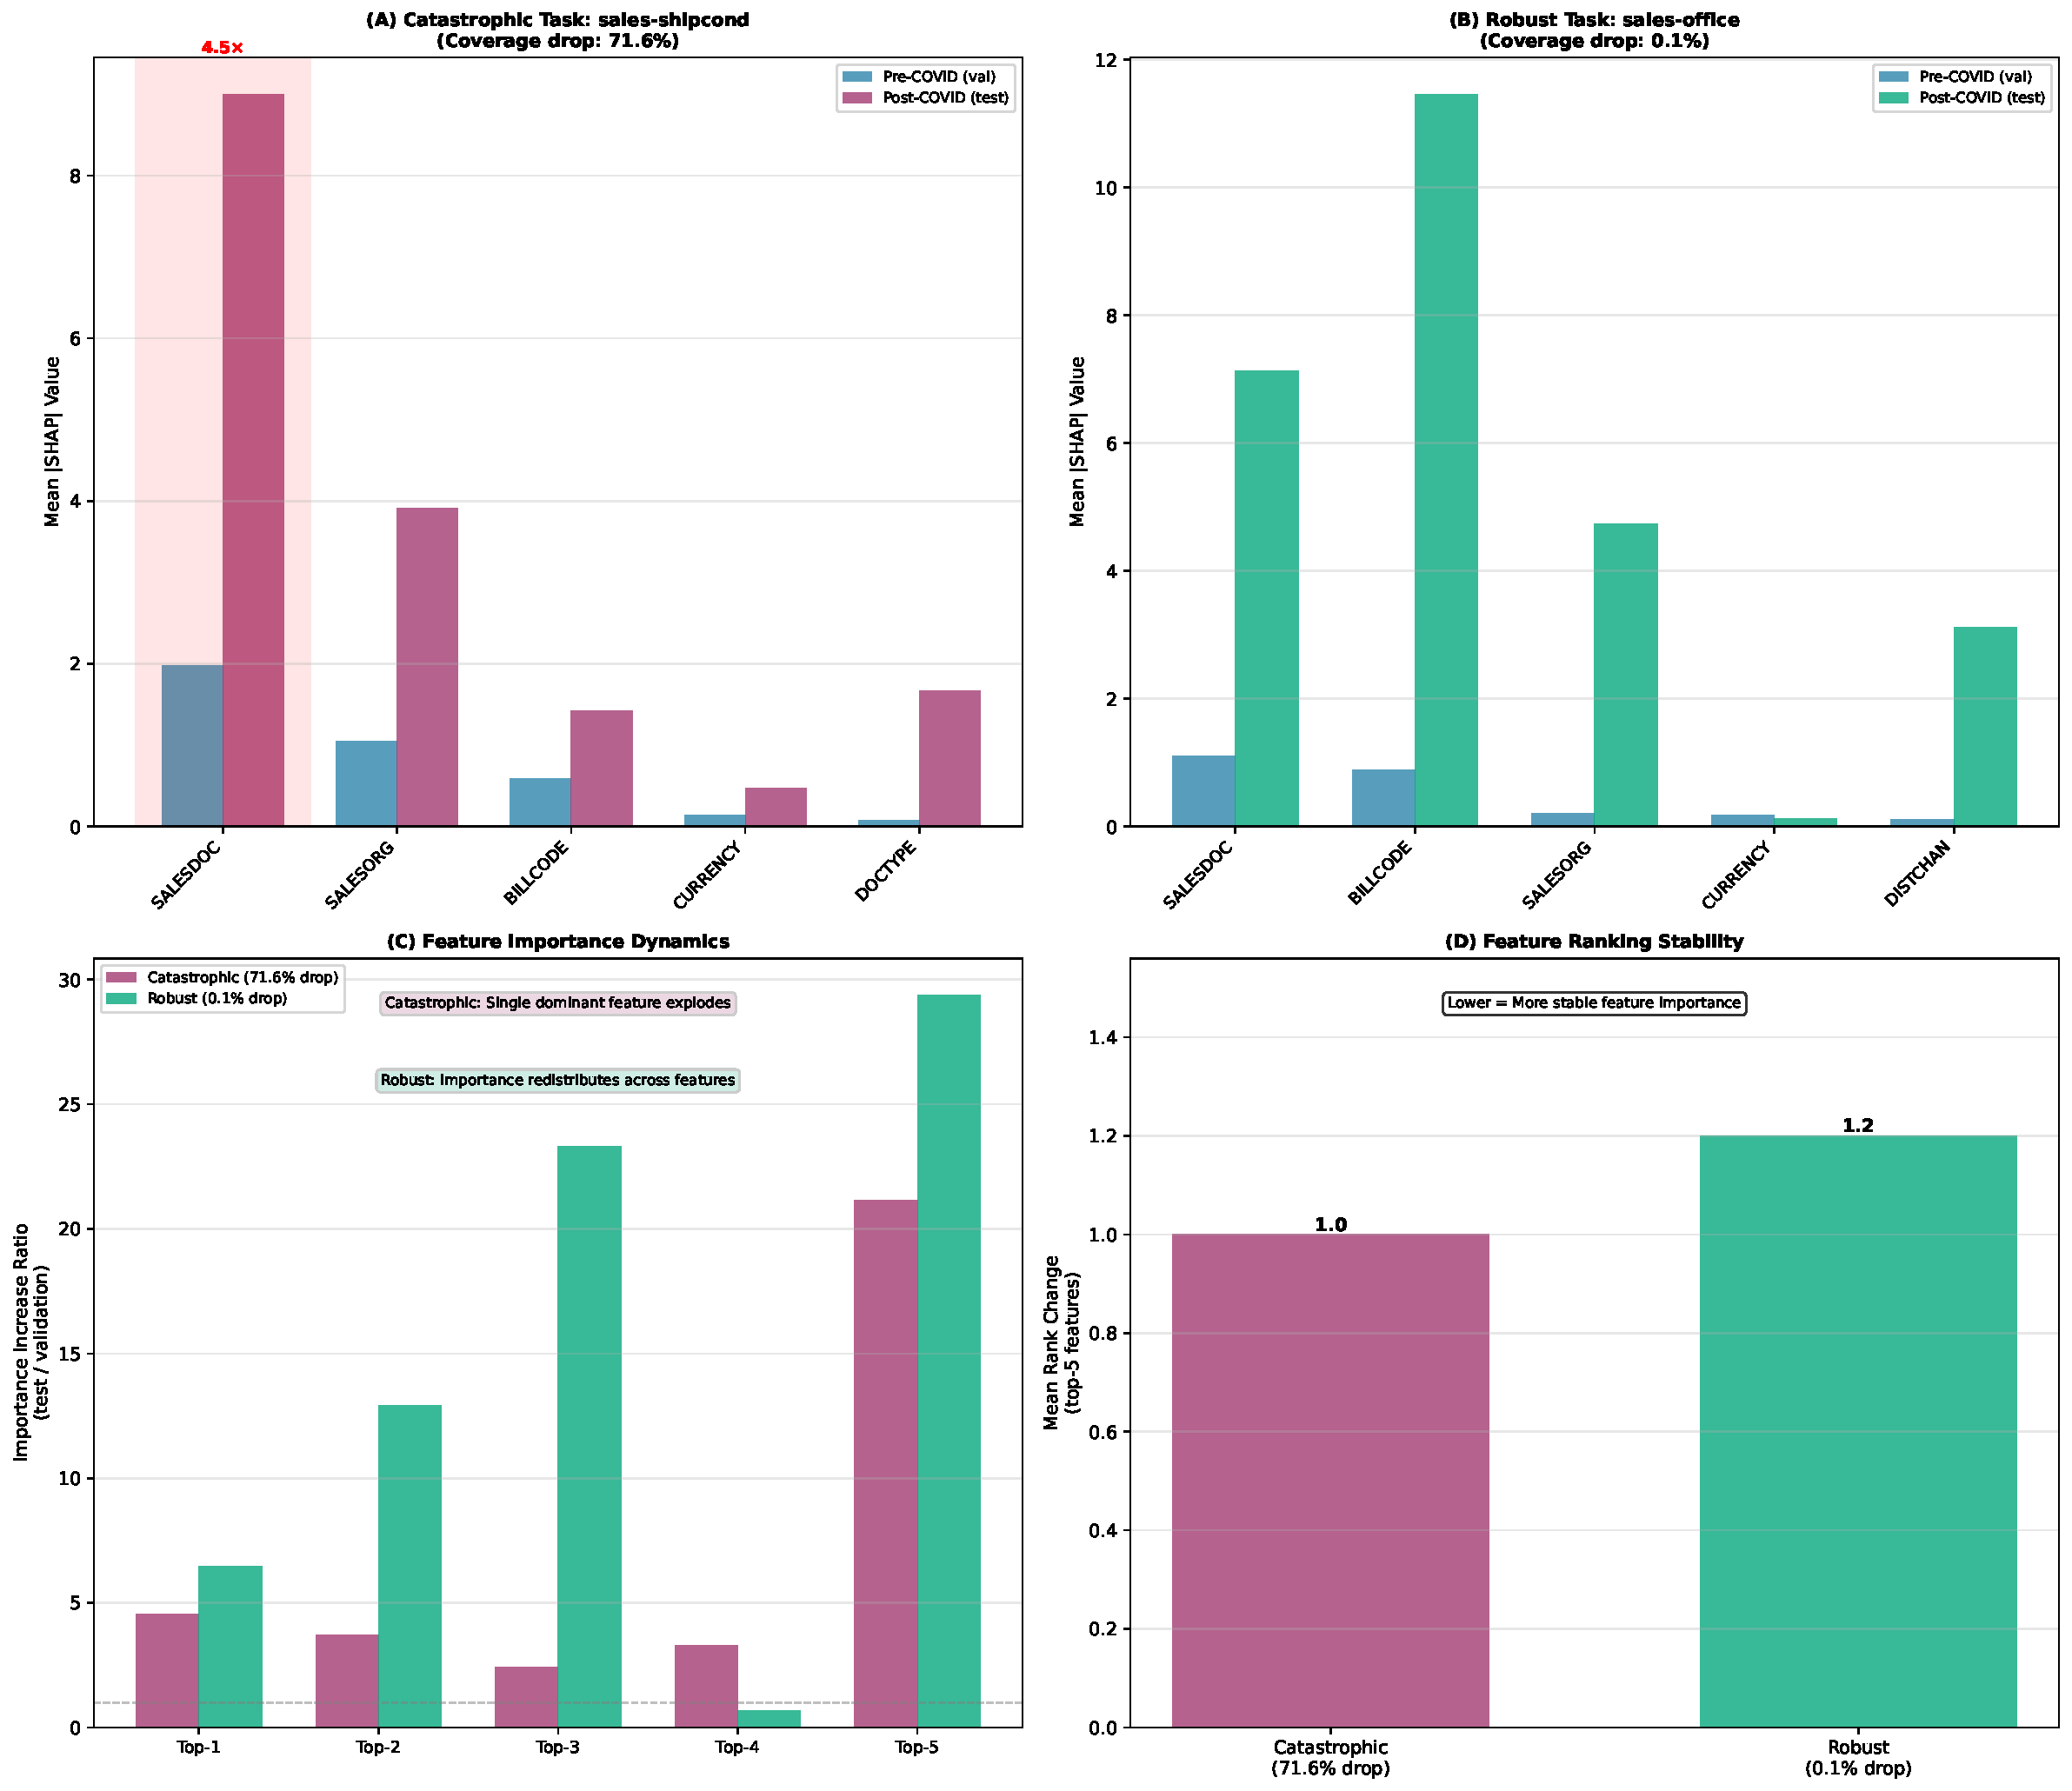
\includegraphics[alt={SHAP concentration trajectory and coverage response},width=\columnwidth]{../figures/figure3_feature_importance}
\Description{Line chart comparing SHAP top-feature concentration with coverage drop and robustness for sample cases.}
\caption{Representative SHAP concentration dynamics under shift. Concentrated single-feature dependence leads to catastrophic coverage loss, while dispersed importance is safer.}
\label{fig:shap}
\end{figure}

\begin{figure}[t]
\centering
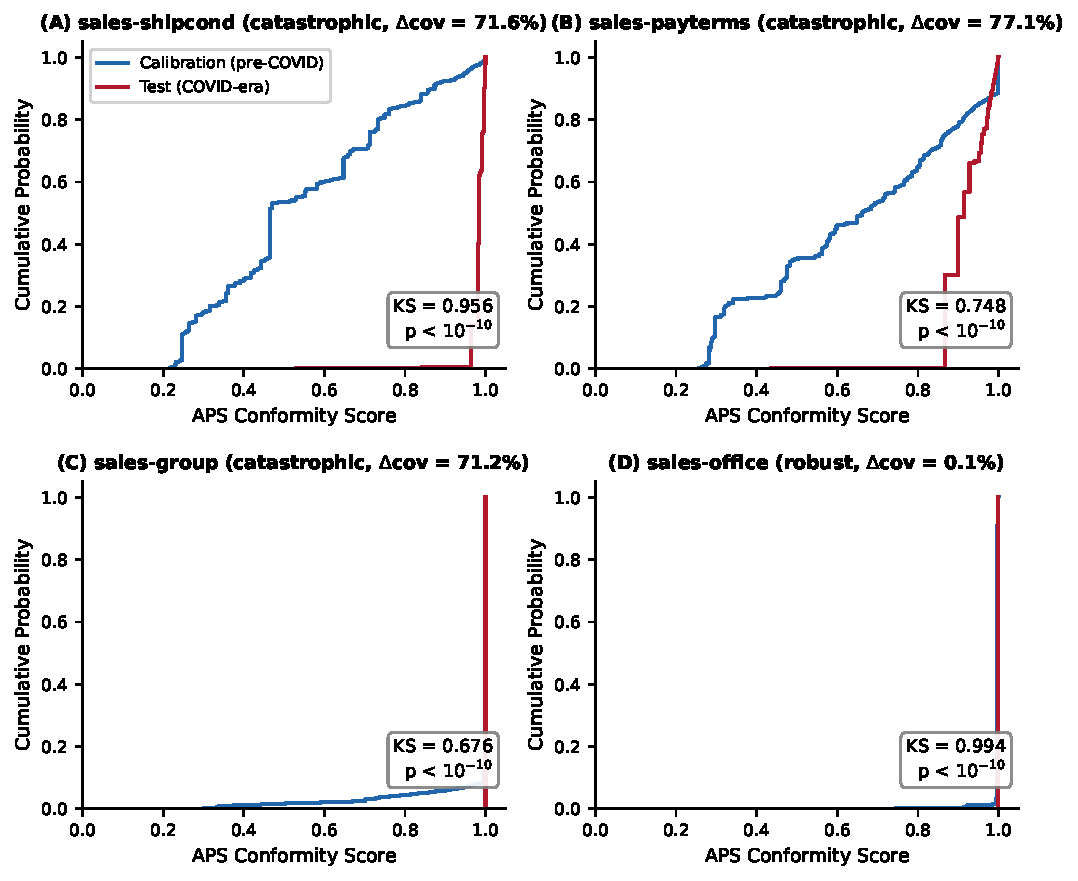
\includegraphics[alt={Conformity score CDF comparison},width=\columnwidth]{../figures/conformity_score_cdfs}
\Description{Two-panel CDF plots for conformity scores comparing calibration and test distributions under shift.}
\caption{Conformity score CDFs under calibration and test (seed=42). Right-shifts in catastrophic settings mean higher score requirements for the true label.}
\label{fig:cdf}
\end{figure}

\subsection{Mechanism checks}
Three observations support mechanism-level interpretation:
\begin{enumerate}
\item Catastrophic tasks show strong right-shifts in APS score CDFs (higher scores needed for the true label).
\item SHAP concentration is stable under resampling (within-task coefficient variation below 1\%).
\item Seed instability appears mostly in edge cases where top feature identity shifts, not in robust low-concentration tasks.
\end{enumerate}

\section{Decision Guidance}
We propose an exploratory protocol:
\begin{itemize}
  \item \textbf{Compute} SHAP concentration on validation data.
  \item If $C\le 40\%$, treat as lower-risk.
  \item If $C>40\%$, check for protective secondary features and model-specific stability.
  \item In ambiguity band 35--45\% or unstable concentration, use conservative monitoring and do not assume robustness.
\end{itemize}

For intermediate and high $C$, retraining can recover part of the loss in some tasks, and ACI/RAPS can be complementary but not universally effective.

\section{External Validation}
In 9 external held-out domains (16 multiclass tasks total), concentration remains associated with failure severity. Covertype is consistently catastrophic with high concentration; many low-concentration datasets remain robust. Boundary cases (e.g., KDDCup99) show intermediate variability, motivating uncertainty bands and post-hoc calibration.

\section{Discussion and Limitations}
\begingroup
\hbadness=10000
\begin{sloppypar}
\begin{raggedright}
Coverage degradation risk is model-specific and mechanism-dependent. SHAP concentration explains when failure is amplified through concentrated dependence, but does not replace full monitoring.
Evidence is strongest for gradient-boosted trees and current seeds.
Transfer across model classes is partial.
\textbf{Limitations.} Current evidence is strongest for multiclass tasks and this experimental protocol. Binary settings and some model classes may behave differently.
Exploratory thresholds should be revalidated before deployment and are not intended as a universal rule.
\end{raggedright}
\end{sloppypar}
\endgroup

\section{Conclusion}
Across extensive 50-seed experiments and external validation, SHAP concentration is a practical pre-deployment indicator of conformal vulnerability under shift. We provide an exploratory diagnostic and a conservative thresholding workflow; we deliberately avoid causal claims and avoid overgeneralization beyond the observed mechanism.

\bibliography{../uai_2026/references}

\end{document}
